\subsection{Versionskontrolle mit Git}
\subsubsection{Allgemein}
% TODO: Quelle
% - https://www.atlassian.com/de/git/tutorials/what-is-version-control#:~:text=Die%20Versionskontrolle%2C%20auch%20bekannt%20als,Quellcode%20im%20Zeitverlauf%20verwalten%20k%C3%B6nnen.
% - https://www.dev-insider.de/was-ist-versionskontrolle-a-701050/

Die Versionskontrolle oder Quellcodekontrolle ermöglicht es Änderungen an
Softwarecode zu verfolgen. Die Verfolgung aller Änderungen erlaubt bei Bedarf
die Wiederherstellung eines früheren Datenstands.

Versionskontrollsysteme, wie Git, speichern jede Änderung am Code in speziellen
git-Datenbank-Dateien. Programmierer können dadurch in ihren Teams genau
analysieren, wer welche Zeile wann geändert oder neu eingesetzt hat.

Durch Git können mehrere Entwickler an demselben Projekt bzw. Repository
arbeiten und sogar dieselben Dateien ändern. Git bietet hierfür Prozesse um
solche Konflikte sauber lösen zu können. Beim Zusammenführen der beiden
Zustände, kann man entscheiden welche Zeile man aus welcher Änderung übernimmt.

Git bietet durch die Speicherung jeder Änderung nicht nur den Vorteil vom
gemeinsamen Arbeiten, sondern auch eine Art \glqq Backup\grqq{}. Durch den
genauen Verlauf des Quellcodes, können Fehlerursachen schneller analysiert,
gefunden und verifiziert werden. Um die einzelnen Snapshots bzw. Schnappschüsse
des aktuellen Standes zu markieren, gibt es in Git die sogenannten Commits.

Die folgenden Begriffsklärungen rund um Git sind wichtig, um den Rest der Arbeit
besser zu verstehen.

\subsubsection{Repositories und Commits}
Das Git-Repository ist der Kern des Projekts und umfasst alle Dateien, die von
Git getracked werden sollen. Es ist sozusagen das Projekt an dem die Entwickler
arbeiten. Um ein Repository anzulegen braucht es nur einen Ordner in dem man
in der Konsole folgenden Befehl ausführt:
\begin{lstlisting}[style=Bash]
    $ git init
\end{lstlisting}
Daraufhin wird in diesem Verzeichnis ein neuer \texttt{.git}-Ordner erstellt,
welcher alle Informationen über das gerade erstellte Repository enthält. Sobald
man nun beispielsweise eine neue Textdatei anlegt, wird die Handlung im
\texttt{.git}-Ordner getracked.

Git arbeitet mit Snapshots, die man manuell anlegen muss. Wenn der Entwickler
nun täglich einen Absatz in die Textdatei schreibt, gibt es hierfür keine
Historie. Git weiß nur, dass im ersten Snapshot keine Datei vorhanden war und
nun eine Datei mit gefülltem Text vorliegt. Um einen Verlauf der Erstellung
zu speichern, muss der Entwickler sogenannte Commits erstellen. Wann die Commits
jeweils erstellt werden müssen, ist dem Entwickler selbst überlassen. In diesem
Fall kann er beispielsweise nach jedem Absatz einen Commit erstellen. Zuerst
kann er in der Konsole alle geänderten Dateien abfragen mit:

\begin{lstlisting}[style=Bash]
    $ git status
\end{lstlisting}

Die Ausgabe sieht in dem Beispiel dann ungefähr so aus:

\begin{lstlisting}[style=Bash]
    On branch main

    No commits yet

    Untracked files:
    (use "git add <file>..." to include in what will be committed)
        hallo-welt.txt

    nothing added to commit but untracked files present (use "git add" to track)
\end{lstlisting}

\newpage
Wie die Ausgabe bereits verrät, wurde bisher noch kein Commit angelegt. Außerdem
verrät sie, dass die Datei \texttt{hallo-welt.txt} angelegt wurde, bisher jedoch
nicht getracked wird. Nun kann der Entwickler die Änderung tracken, indem er
folgenden Befehl ausführt:

\begin{lstlisting}[style=Bash]
    $ git add hallo-welt.txt
\end{lstlisting}

Durch den Befehl \code{git add .} kann er auch mit einem Befehl alle
\glqq untracked\grqq{} Änderungen in den neuen Commit hinzufügen. Jetzt weiß
Git welche Änderungen commited werden sollen. Mit dem Befehl

\begin{lstlisting}[style=Bash]
    $ git commit -m "Neue Hallo Welt Datei angelegt"
\end{lstlisting}

wird ein Commit mit der Nachricht \glqq Neue Hallo Welt Datei angelegt\grqq{}
angelegt. Dies ist nun ein neuer Snapshot, welcher in der Commit-Historie
gespeichert wird. Sollte der Programmierer die Datei nun verändern, kann er die
neuen Änderungen erneut tracken und wieder committen. An diesem Punkt könnte er
jedoch jederzeit zu dem alten bereits committeten Zustand zurückkehren.

Damit Repositories im Internet verfügbar sind, benötigt man einen Server auf dem
eine Version des lokalen Repositories gespeichert ist. Diese Repositories nennt
man auch Remote-Repositories. Der bekannteste Dienstleister für die Speicherung
von Remote-Repositories ist GitHub. Der Vorteil von einer Online-Version des
eigenen Repositories ist, dass andere Entwickler das Projekt klonen und
schließlich mitarbeiten können. Nach dem Klonvorgang haben diese Personen
ebenfalls eine lokale Kopie des Repositories auf ihrem Endgerät. Um nun einen
lokalen Commit online verfügbar zu machen, muss dieser \emph{gepushed} werden.
Zuerst muss über folgenden Befehl geprüft werden, ob im lokalen Repository das
richtige Remote-Repository referenziert wird:

\begin{lstlisting}[style=Bash]
    $ git remote -v
    origin	https://github.com/user/repository-name (fetch)
    origin	https://github.com/user/repository-name (push)
\end{lstlisting}

Sollten die Adressen zum richtigen Online-Repository verweisen, kann mit
folgendem Befehl ein Commit hochgeladen werden:

\begin{lstlisting}[style=Bash]
    $ git push
\end{lstlisting}

Um mögliche Änderungen durch andere Mitarbeitende in das lokale Repository zu
laden benötigt man einen sogenannten \emph{Pull}:

\begin{lstlisting}[style=Bash]
    $ git pull
\end{lstlisting}

Der Git-Workflow umfasst noch viele weitere Befehle und kann für Unerfahrene
schnell sehr kompliziert werden. Aus diesem Grund enthalten die meisten gängigen
Entwicklungsumgebungen grafische Oberflächen für die Verwendung von Git. So
benötigt der Entwickler weder Konsole, noch tieferes Fachwissen über die genaue
Verwendung der Befehle.

\subsubsection{Branches}
Git bietet neben der Kontrolle und Verfolgung von Commits und Änderungen auch
die Möglichkeit echt parallel zu arbeiten. In einem großen Softwareprojekt gibt
es neben der Entwicklung von neuen Features meist auch zur Laufzeit auftretende
Fehler, welche Behoben werden müssen.

In diesem beispielhaften Fall, dass in einer Software ein gravierender Fehler
auftritt, sollte möglichst schnell ein Update mit einer Lösung ausgearbeitet
werden. Es kann jedoch sein, dass ein Teil des Entwicklungsteam gerade an einem
sehr großen neuen Feature arbeitet, welches nicht halbfertig veröffentlicht
werden darf. Es muss also eine Lösung geben, dass eine neue Version mit dem
behobenen Fehler veröffentlicht werden kann, ohne, dass die Arbeit an dem neuen
Feature gestört oder rückgängig gemacht werden muss. Git stellt mit dem Konzept
von Branches eine Lösung für dieses Problem dar.

\begin{figure}[h]
    \centering
    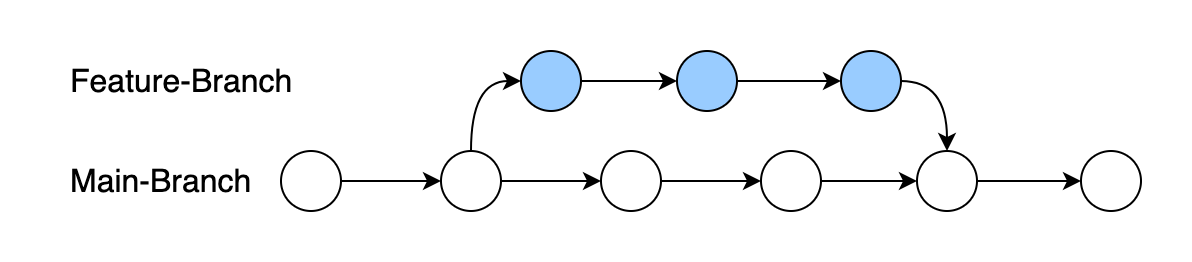
\includegraphics[width=\textwidth]{git-branch}
    \caption{Git: Branches}
    \bildquelle{Eigene Darstellung}
    \label{fig:git-branch}
\end{figure}

Branches (dt. Äste) teilen den linearen Entwicklungsablauf in mehrere parallele
Zustände. Standardmäßig arbeitet man bei Git auf dem \texttt{Main}-Branch. Der
Hauptzweig sozusagen (siehe Abbildung \ref{fig:git-branch}, der weiße Strang).
Die weißen Kugeln stellen in Abbildung \ref{fig:git-branch} jeweils einzelne
Commits dar. Sobald ein neues Feature entwickelt wird, möchte der zuständige
Programmierer nicht, dass sich während der Entwicklung etwas am
restlichen Code ändert. Aus diesem Grund eröffnet der Feature-Programmierer, wie
in Abbildung \ref{fig:git-branch} ersichtlich, einen neuen Branch auf den
aktuellen Commit des Hauptzweigs. Wenn sich der Hauptzweig jetzt durch
Änderungen von anderen Kollegen ändert, merkt der Feature-Programmierer nichts
davon, weil er sich auf einem neuen Ast befindet und dabei seine ganz eigene
Kopie des Projekts bearbeitet. Sobald er mit dem Feature fertig ist, kann er
seinen Branch mit dem \texttt{Main}-Branch wieder zusammenführen. Falls sich in
der Zwischenzeit die Dateien und Zeilen, die er auch bearbeitet hat, geändert
haben, müssen die Konflikte in aller Regel manuell gelöst werden. Sollten nicht
dieselben Zeilen bearbeitet worden sein, löst Git die Konflikte selbst und führt
die zwei Zustände selbst zusammen.

Eine bekannte Konvention unter Programmierern ist es, dass der
\texttt{Main}-Branch immer eine lauffähige Version der Software hält. Es darf
nie ein nicht-kompilierbarer oder unfertiger Stand auf dem Hauptzweig landen.
So stellt man sicher, dass neue abzweigende Branches immer auf einer
lauffähigen Basis aufbauen.

\begin{figure}[H]
    \centering
    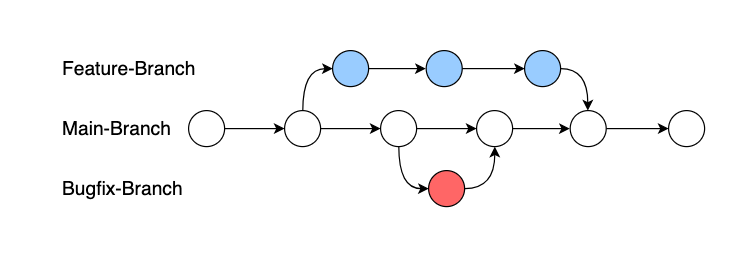
\includegraphics[width=\textwidth]{git-branch-fehler}
    \caption{Git: Branches (Bugfix-Branch)}
    \bildquelle{Eigene Darstellung}
    \label{fig:git-branch-fehler}
\end{figure}

Wie in Abbildung \ref{fig:git-branch-fehler} zu erkennen, werden auch Bugfixes
meist in einem anderen Branch behandelt. Nun lässt sich auch die anfangs
erläuterte Problemstellung leicht erklären. Wenn ein gravierender Softwarefehler
auftritt, kann das Team ausgehend vom lauffähigen \texttt{Main}-Branch einen
neuen Zweig zur Fehlerbehebung eröffnen (siehe Abbildung
\ref{fig:git-branch-fehler}, roter Kreis). Auf diesem Zweig können sie
unabhängig von der Entwicklung eines neuen Features den Fehler beheben, mit dem
Hauptzweig zusammenführen und das Update veröffentlichen. Wenn das Feature
fertig ist, wird es mit dem Hauptzweig zusammengeführt und der Fehler auch darin automatisch behoben. Sollte der Fehler so gravierend sein, dass er die
Entwicklung des \texttt{Feature}-Branches hindert, kann man jederzeit den
\texttt{Main}-Branch in den \texttt{Feature}-Branch mergen und den
\texttt{Feature}-Branch somit wieder auf den aktuellen Stand bringen. Mergen
heißt hier nichts anderes als das Zusammenführen zweier Codebasen. Dies ist auch
sinnvoll, wenn die Entwicklung eines Features einen längeren Zeitraum
beansprucht. Ansonsten geht man die Gefahr ein, dass sich der Hauptzweig bei der
Zusammenführung so sehr verändert hat, dass er dem \texttt{Feature}-Zweig zu
sehr differenziert und eine Zusammenführung sehr viel manuelle Arbeit erfordert.
